\begin{figure}
  \resizebox{\columnwidth}{!}{%
    \begin{tikzpicture}
      % Actors
      \node[label=Alice] (alice) at (0,0) {
\includegraphics[height=4cm]{img/alice.png}};
      \node[label=Bob] (bob) at (24,0) {
\includegraphics[height=4cm]{img/bob.png}};
      \node[label=Eve] (eve) at (12,-4) {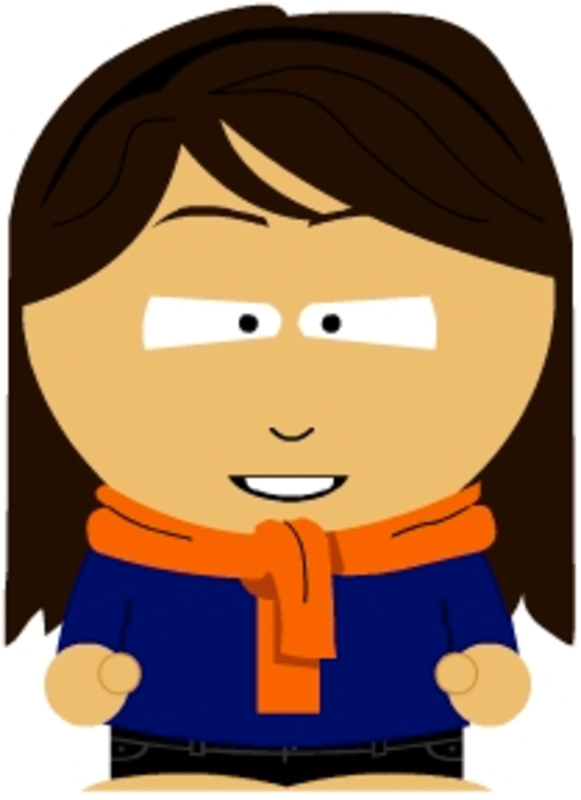
\includegraphics[height=4cm]{img/eve.png}};

      % Canal
      \draw (4,0) ellipse (0.35 and 0.5);
      \draw (20,-0.5) arc (-90:90:0.5);
      \draw (4,0.5) -- ++(16,0);
      \draw (4,-0.5) -- ++(16,0);
      \node (label) at (12, 1) {Canal de communication non sécurisé};

      \draw[->] (eve.west) -- ++(-1.5,0) -- node[left] {Écoute} ++(0,3.5);
      \draw[->] (eve.east) -- ++(1.5,0) --  node[right] {Modifie} ++(0,3.5);

    \end{tikzpicture}%
  }

  \caption{Modèle de canal de communication non sécurisé}
\end{figure}